% SPDX-License-Identifier: CC-BY-4.0
\documentclass[11pt,a4paper]{article}
\usepackage[left=20mm,right=20mm,top=18mm,bottom=18mm,headheight=15pt]{geometry}
\usepackage{fontspec}
\setmainfont{DejaVu Serif}[AutoFakeSlant=0.2]
\setsansfont{DejaVu Sans}
\setmonofont{DejaVu Sans Mono}[Scale=0.85]
\usepackage{polyglossia}
\setdefaultlanguage{russian}
\setotherlanguage{english}
\usepackage{amsmath,amssymb,booktabs,tabularx,graphicx,xcolor,fancyhdr}
\usepackage{ragged2e}
\usepackage[font=small,labelfont=bf]{caption}
\usepackage{float}
\usepackage[unicode,colorlinks=true,linkcolor=teal,urlcolor=teal,citecolor=teal]{hyperref}
\hypersetup{pdftitle={Многомерные пространства, тени и миры вспышек},pdfauthor={Вадим}}
\graphicspath{{../figures/}}
\setlength{\parindent}{0pt}
\setlength{\parskip}{4pt}
\setlength{\emergencystretch}{3em}
\setlength{\textfloatsep}{10pt plus 2pt minus 2pt}
\setlength{\intextsep}{10pt plus 2pt minus 2pt}
\renewcommand{\topfraction}{0.9}
\renewcommand{\textfraction}{0.1}
\renewcommand{\floatpagefraction}{0.75}
\clubpenalty=10000
\widowpenalty=10000
\pagestyle{fancy}
\fancyhf{}
\fancyhead[L]{\small\sffamily Пространства, тени и миры вспышек}
\fancyhead[R]{\small\sffamily Версия 1.0.0}
\fancyfoot[L]{\small\sffamily Исследовательский пакет · 10.10.2026}
\fancyfoot[R]{\small\thepage}
\newcommand{\code}[1]{\texttt{\detokenize{#1}}}
\newcommand{\status}[1]{\textbf{#1}}
\begin{document}
\raggedright
\thispagestyle{empty}
{\LARGE\sffamily\bfseries Многомерные пространства,\par тени и миры вспышек\par}
\vspace{3mm}
{\large Точная проверка и воспроизводимые эксперименты\par}
\vspace{2mm}
Вадим \hfill 10 октября 2026 года · версия 1.0.0

\textbf{Аннотация.} Числа представляются координатами степеней простых, а составные адреса -- объединением теней произведений. Из этой картины получается точный поиск в конечных мирах: проверяется короткое окно, сохраняются адреса и доказательства составности, следующая опора выбирается по крайней пустоте. Пакет содержит доказательства базовых тождеств, программы, исходные измерения, повторные запуски и их ограничения. Для кандидата $3P-82$ подтверждено отсутствие делителей до миллиона; его простота не установлена.

\section{Координаты, слои и тени}

Каждому простому сопоставляется ось, а показателю его степени -- координата. Например, $60=2^2\cdot3\cdot5$ имеет координаты $(2,1,1)$ на осях $2,3,5$. Умножение складывает координаты; единица соответствует нулевому вектору. Эта модель опирается на единственность разложения на простые множители.

При границе $X$ координатный мир имеет вид
\[
 H_r(X)=\left\{\prod_{i=1}^{r}p_i^{e_i}\le X:\ e_i\ge0\right\}.
\]
Зафиксируем степень последней оси $q=p_r$: $e_r=k$. Такой слой, или «блин», состоит из чисел $q^k m$. Его проекция после удаления множителя $q^k$ в точности равна
\[
 H_{r-1}\!\left(\left\lfloor X/q^k\right\rfloor\right).
\]
Доказательство -- равносильность $q^k m\le X$ и $m\le\lfloor X/q^k\rfloor$. Комплексный вес также раскладывается точно: $(q^k m)^{-s}=q^{-ks}m^{-s}$. Но численная компенсация весов сама по себе не удостоверяет отсутствие точек.

В вычислении на числовой оси \emph{тень простого} означает составные адреса, кратные этому простому. Пересечения теней соответствуют повторному покрытию одного адреса. Для поиска пустот достаточно знать, занят ли адрес; число покрывающих его слоёв -- отдельная характеристика.

\begin{figure}[!htbp]
\centering
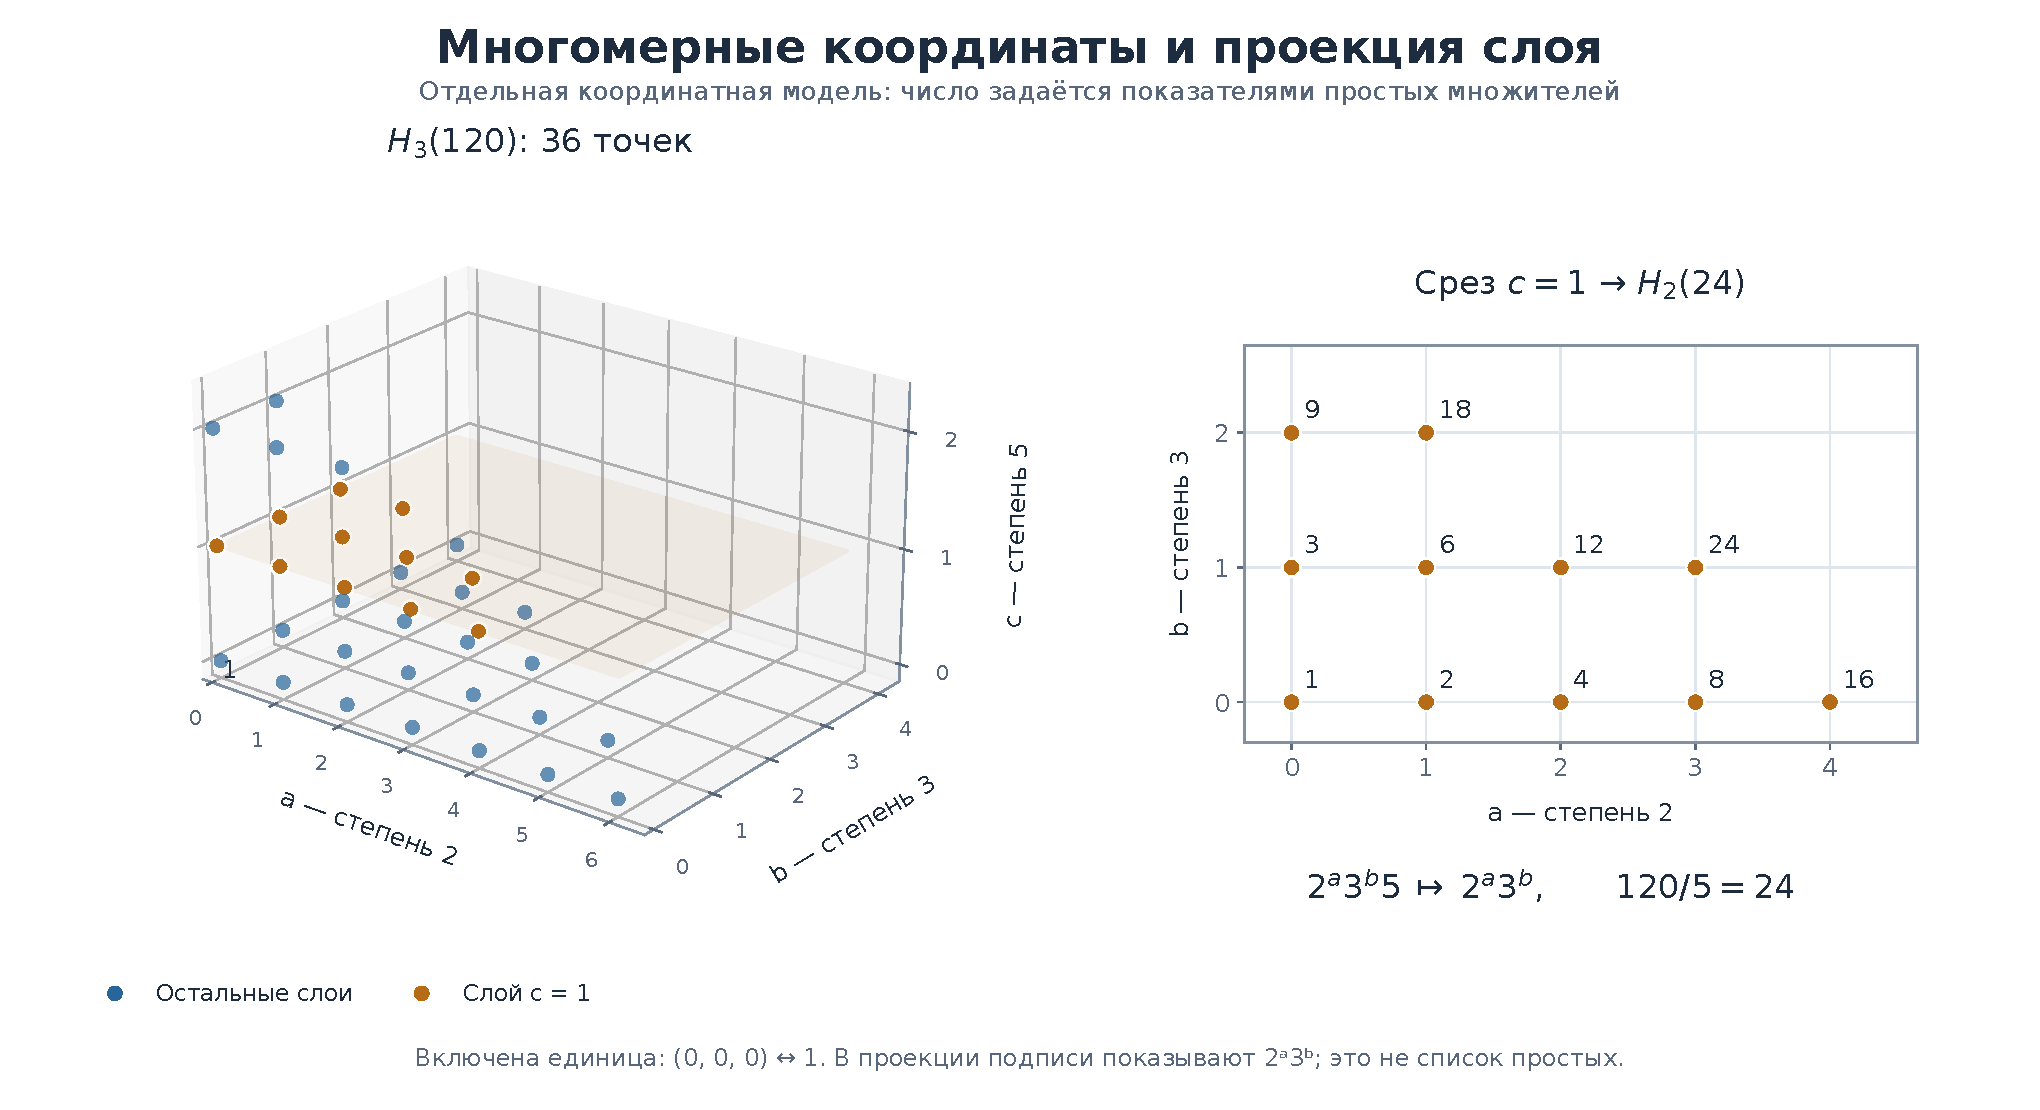
\includegraphics[width=\linewidth]{prime_space_projection.pdf}
\caption*{Срез по степени пятёрки $k=1$ в $H_3(120)$ проецируется в $H_2(24)$. Координатный мир $H_r$ и конечный мир произведений $S_B$ ниже имеют разные определения.}
\end{figure}

\section{Конечный мир, вспышка и точная обрезка}

Для нечётного $B\ge3$ зададим
\[
S_B=\{pm:\ p\le B\text{ -- нечётное простое},\quad
             m\text{ нечётно},\ 3\le m\le B\},
\]
\[G(B)=\min(B^2,3B+4).\]
Мир $S_B$ состоит из различных занятых адресов, без кратностей. $G(B)$ -- \textbf{гарантированная граница точного поиска}, а не утверждение о максимально возможной границе покрытия.

\textbf{Утверждение.} На нечётных адресах $3\le n\le G(B)$ пустоты $S_B$ в точности совпадают с простыми.

\textbf{Доказательство.} Элемент $pm$ составен. Обратно, у нечётного составного $n$ есть наименьший простой делитель $p\le\sqrt n\le B$. Если $m=n/p>B$, то $m\ge B+2$ и $n\ge3(B+2)>G(B)$ -- противоречие. Следовательно, оба множителя допустимы в $S_B$.

\textbf{Вспышка} -- переход от $B$ к крайнему простому в $(B,G(B)]$. Поиск начинается с правого окна из 15 нечётных адресов. Если всё окно закрыто, рассматривается следующее окно слева. Найденный адрес становится новой опорой. Все адреса справа от него уже имеют доказательства составности: это \emph{сертификат закрытого суффикса}. Миры для промежуточных простых не строятся; сама цепочка вспышек не является полным списком простых.

Текущая быстрая реализация сохраняет адреса и их делители непосредственно. Малый базис расширяется только для ещё не исключённого кандидата и только до $\lfloor\sqrt n\rfloor$. Для его построения используется обычное решето. Геометрическая и комплексная картины помогают организовать описание; расчёт комплексных моментов и последующее восстановление адресов в этом ядре не выполняются.

\textbf{Обрезка покрытия.} Пусть $C'\subseteq C$ -- сокращённое покрытие, а $U$ -- остальные сохранённые тени. Тогда
\[
 C'\cup U=C\cup U
 \quad\Longleftrightarrow\quad
 C\setminus C'\subseteq U.
\]
Это проверяется для каждого адреса: удалённое покрытие должно полностью заменяться оставшимися тенями. Поэтому можно не хранить следы вне окна, удалять повторное покрытие и оставлять один делитель на составной адрес.

\textbf{Гарантия точности.} Завершённая проверка полного необходимого набора делителей выявляет любое составное число. При ограниченном базисе отсутствие найденного делителя означает \code{UNKNOWN}. Для объявления простоты необходимы полнота проверки либо другой точный сертификат. Эта гарантия не включает обещание приемлемого времени на произвольно больших числах.

\textbf{Конечная проверка реализации:} 250 миров $B=3,5,\ldots,501$; 94\,873 классификации против независимого решета; 742 окна обрезки; 10\,000 координатных разложений; 48 координатных миров и 134 слоя. Эти испытания проверяют реализацию. Общие утверждения обосновываются приведёнными выше доказательствами.

\section{Рябь: какие старые тени ещё нужны}

Вопрос о глубине истории относится к \emph{остаткам теней после перекрытия}. Для простого $p\le B$ обозначим его след в окне через $T_p(I)=\{pm\in I:3\le m\le B,\ m\text{ нечётно}\}$. После всех более поздних простых осей остаётся
\[
 \mathcal R_{p,B}(I)=T_p(I)\setminus\!\bigcup_{p<q\le B}T_q(I)
 =\{n\in I:\ n\text{ составно},\ P^+(n)=p\},
\]
где объединение идёт по простым $q$, а $P^+(n)$ -- наибольший \emph{простой} делитель. Равенство справедливо в безопасном окне $I\subseteq[3,G(B)]$.

Действительно, если у $n=pm$ есть простой делитель $q>p$, то $q\mid m$, $q\le B$ и $3\le n/q<m\le B$: более поздняя тень его поглощает. Обратно, в безопасном окне наибольший простой делитель допустим в мире и не имеет более позднего конкурента.

Это возвращает нас к исходным «блинам». Пусть $\mathcal H_{<p}(Y)$ состоит из единицы и произведений меньших нечётных простых, не превосходящих $Y$. При $I=[L,R]$:
\[
 \mathcal R_{p,B}(I)=
 \left(I\cap\bigsqcup_{k\ge1}p^k\mathcal H_{<p}(R/p^k)\right)\setminus\{p\}.
\]
Слои не пересекаются: $k$ -- точная степень $p$. \textbf{Тень не нужна в данном окне, когда ни один её остаточный слой туда не попадает.} Правило и область его применимости можно сохранять вместо повторного обхода всех периодов. Само тождество ещё не даёт быстрого алгоритма проверки непустоты слоя при огромном $P$.

\textbf{Сертификат поглощения целого блока осей.} Снимем из адреса все степени простых до $Y$:
\[
 D_Y(n)=\prod_{p\le Y}p^{v_p(n)}.
\]
Если $D_Y(n)<n$, остаток $n/D_Y(n)>1$ не имеет простых делителей до $Y$ и потому содержит простой делитель $q>Y$. Для составного адреса в безопасном окне это допустимая поздняя ось. Значит, если неравенство проверено на всём окне, \emph{все старые оси до $Y$ поглощены}. Знать конкретные поздние делители для этого вывода не требуется. Полные степени $v_p$ необходимы: один найденный малый делитель такого вывода не даёт.

Если покрытие требуется сохранять \emph{полным непрерывным суффиксом простых осей}, его самая поздняя левая граница равна
\[
 \boxed{a_* = \min_{\substack{n\in I\\n\text{ составно}}}P^+(n).}
\]
Суффикс $[a,B]$ покрывает все составные адреса тогда и только тогда, когда $a\le a_*$. В пустом от составных окне покрывающие оси не нужны. Разреженный сертификат может хранить только отдельных владельцев, поэтому число всех простых между $a_*$ и $B$ не является оценкой необходимой памяти.

\begin{center}
\begin{tabularx}{\linewidth}{@{}r r X r@{}}
\toprule
Мир $B$ & $a_*$ & Осей в полном суффиксе & Сохранено владельцев\\
\midrule
6\,053 & 31 & 780 & 13\\
490\,057 & 137 & 40\,740 & 12\\
4\,410\,517 & 2\,213 & 309\,686 & 12\\
\bottomrule
\end{tabularx}
\end{center}
Это точные результаты для 15 нечётных адресов у правой границы. Пилот проверил 14 миров канонической цепочки и 668 простых опор до 5000; выполнено 13\,099 проверок равенства остатка и слоя. Граница здесь получена \emph{после полной факторизации малых адресов}; это проверка структуры, а не ускорение рекордного поиска. Набор владельцев в таблице не объявляется минимальным покрытием.

Поглощение может смениться возвращением. В мире 71, в окне $[189,217]$, тень 5 равна $\{195,205,215\}$ и поглощается осями 13, 41 и 43. Настоящая следующая вспышка даёт 211. В её окне $[609,637]$ число $625=5^4$ снова требует ось 5. Этот переход начинается с 71; он не является частью канонической цепочки от 3. Значит, сертификат ненужности должен указывать окно или доказанный диапазон переноса.

\section{Сравнение с решётами и Миллером -- Рабином}

Точные решёта также не принимают составные числа за простые при достаточном базисе. В нашем опыте решето и кандидатный поиск решают одну задачу: найти максимум и закрытый суффикс короткого окна. Полный ряд промежуточных простых не требуется.

Вероятностный Миллер -- Рабин может пропустить составное при неудачном выборе оснований. Для фиксированного нечётного составного вероятность пройти $k$ независимых проверок с равномерно случайными основаниями не превышает $4^{-k}$. Его ответ «составное» достоверен \cite{hac}. Например, $2047=23\cdot89$ проходит основание 2, поскольку $2^{1023}\equiv1\pmod{2047}$. Точная проверка закрывает это число делителем 23.

\textbf{В измерении ниже Миллер -- Рабин точен:} использованы первые 12 простых оснований $2,3,\ldots,37$ и программный запрет $n\ge2^{64}$. Их достаточность следует из результата о наименьшем сильном псевдопростом для этих оснований \cite{sorenson}. Его преимущество во времени в этом опыте получено при сохранении точности.

\begin{center}
\begin{tabularx}{\linewidth}{@{}Xrr@{}}
\toprule
Движок & Исходно, мс & Повтор, мс\\
\midrule
Наш точный кандидатный вариант & 263,506 & 294,488\\
Наше сегментное решето на Python & 713,200 & 826,170\\
Миллер -- Рабин, 12 оснований & 2,035 & 2,219\\
\bottomrule
\end{tabularx}
\end{center}

Протокол: 28 вспышек, 31 различное окно, 12 раундов по три движка; все шесть порядков запуска повторены дважды. Время включает создание движка, необходимый базис и весь общий маршрут. Импорты и независимая сверка выполнены вне таймера. Конечная опора всех маршрутов: $63\,286\,095\,838\,211$.

\begin{figure}[H]
\centering
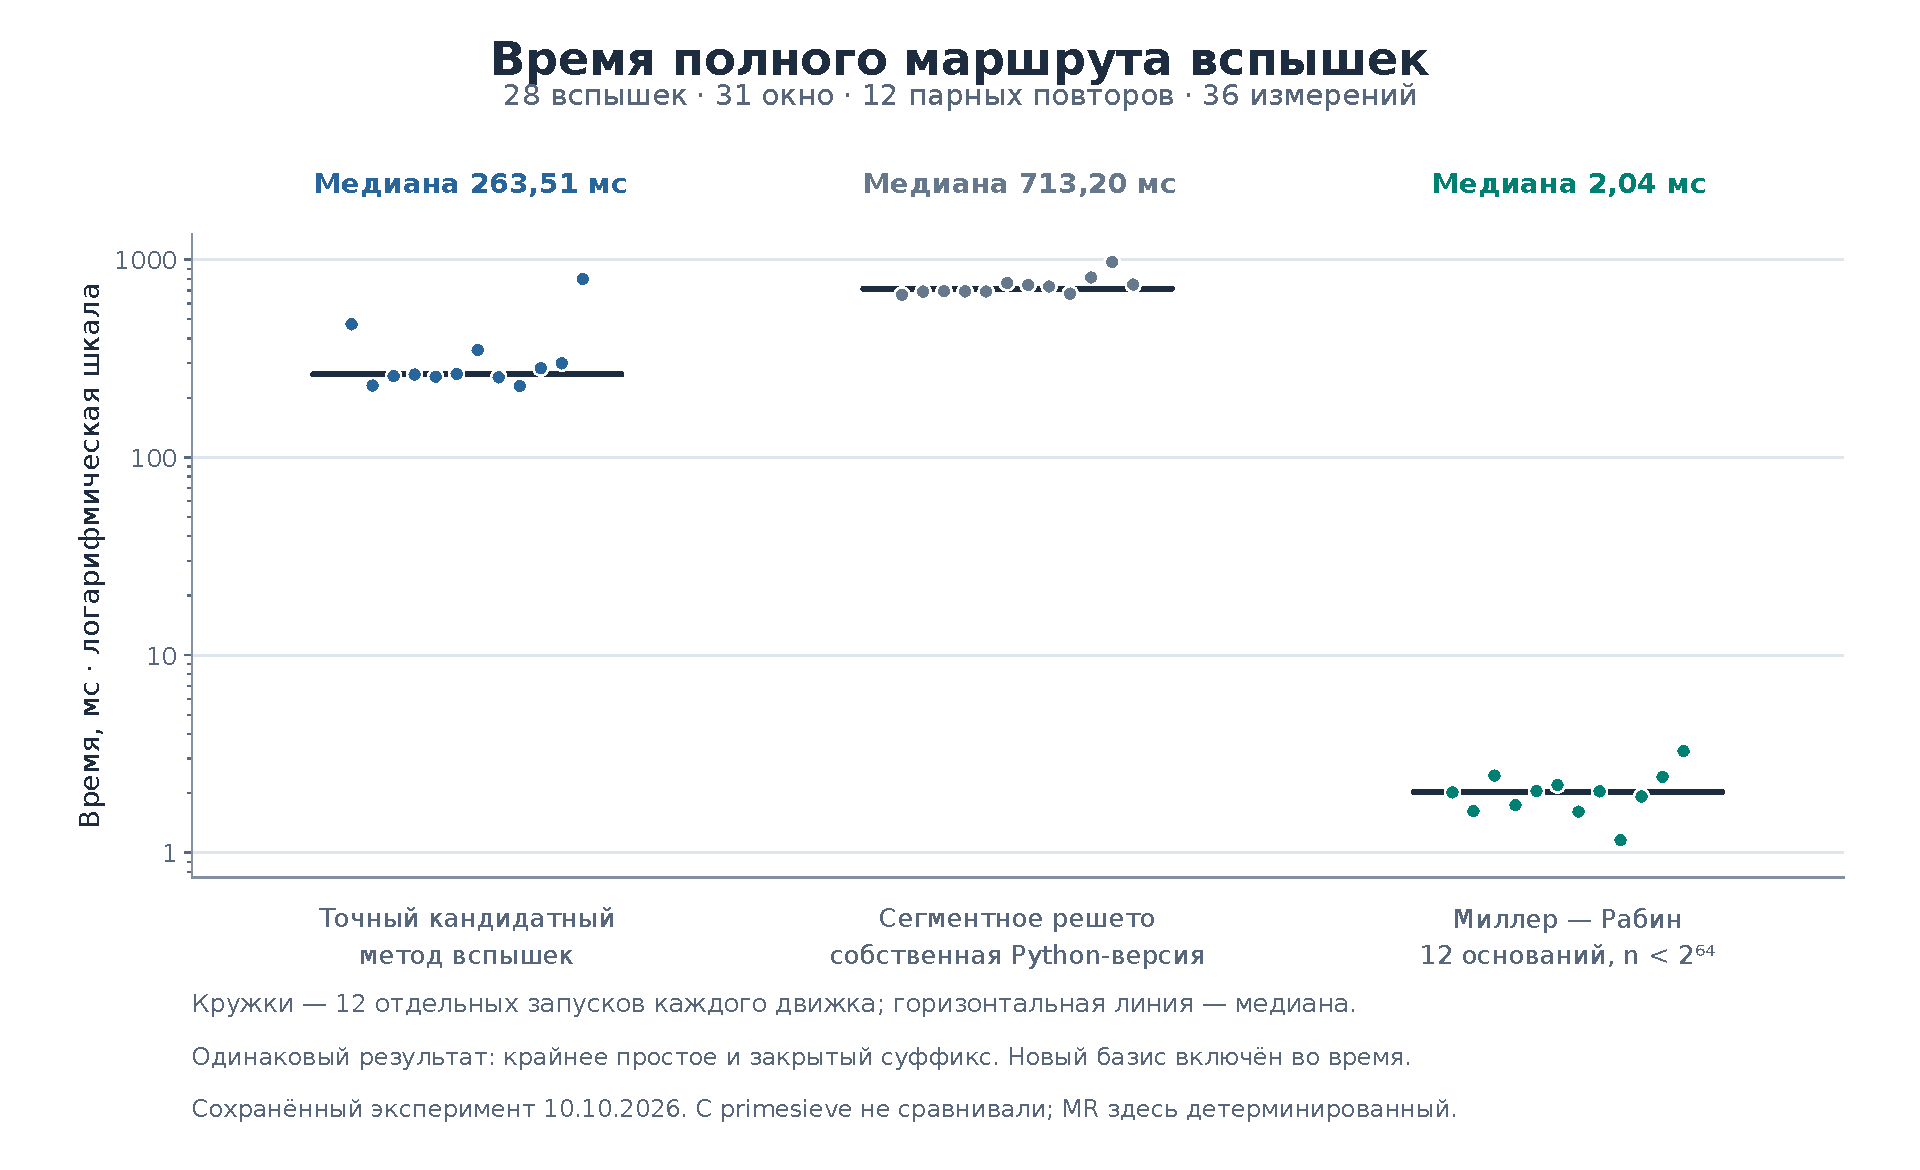
\includegraphics[width=\linewidth]{benchmark_times.pdf}
\caption*{Исходные 36 измерений; шкала времени логарифмическая. Исторические и повторные JSON/CSV сохранены раздельно.}
\end{figure}

По медиане парных отношений наш вариант быстрее Python-сегментного решета в $2{,}79$ раза; точный MR быстрее нашего в $144{,}49$ раза. Это короткое диагностическое сравнение. Производительность оптимизированного C/C++ \code{primesieve} \cite{primesieve} в данном маршруте не измерялась; преимущество над современными решётами в целом не установлено. Стоимость полного перечисления простых также не измеряется этим контрактом.

\section{Как получен кандидат $3P-82$}

За исходное число взято известное простое Мерсенна \cite{gimps}
\[
 P=2^{136\,279\,841}-1,\qquad R=3P+4.
\]
Адреса окна нумеруются от правой границы вниз:
\[
 N_j=R-2j=3P+4-2j=3\cdot2^{136\,279\,841}+1-2j.
\]
Для каждого малого простого $p$ достаточно вычислить
\[
 N_j\bmod p=\bigl(3(2^{136\,279\,841}\bmod p)+1-2j\bigr)\bmod p.
\]
Нулевой остаток даёт точное доказательство составности. Само огромное число в этом опыте не разворачивается.

Проверены все 78\,497 нечётных простых до $10^6$ на 1500 адресах. Найдены делители для 1381 адреса; 119 остались \code{UNKNOWN}. Первые \textbf{43 адреса подряд}, $j=0,\ldots,42$, закрыты. Например, $3P+4$ делится на 53, $3P+2$ -- на 5, $3P$ -- на 3, $3P-80$ -- на 11.

Следующий, 44-й по порядку адрес имеет номер $j=43$:
\[
 \boxed{N_{43}=3P+4-2\cdot43=3P-82
                  =3\cdot2^{136\,279\,841}-85.}
\]
Число 82 получилось из $86-4$. Это наблюдаемое положение кандидата при данном покрытии, а не универсальная постоянная метода.

\begin{figure}[H]
\centering
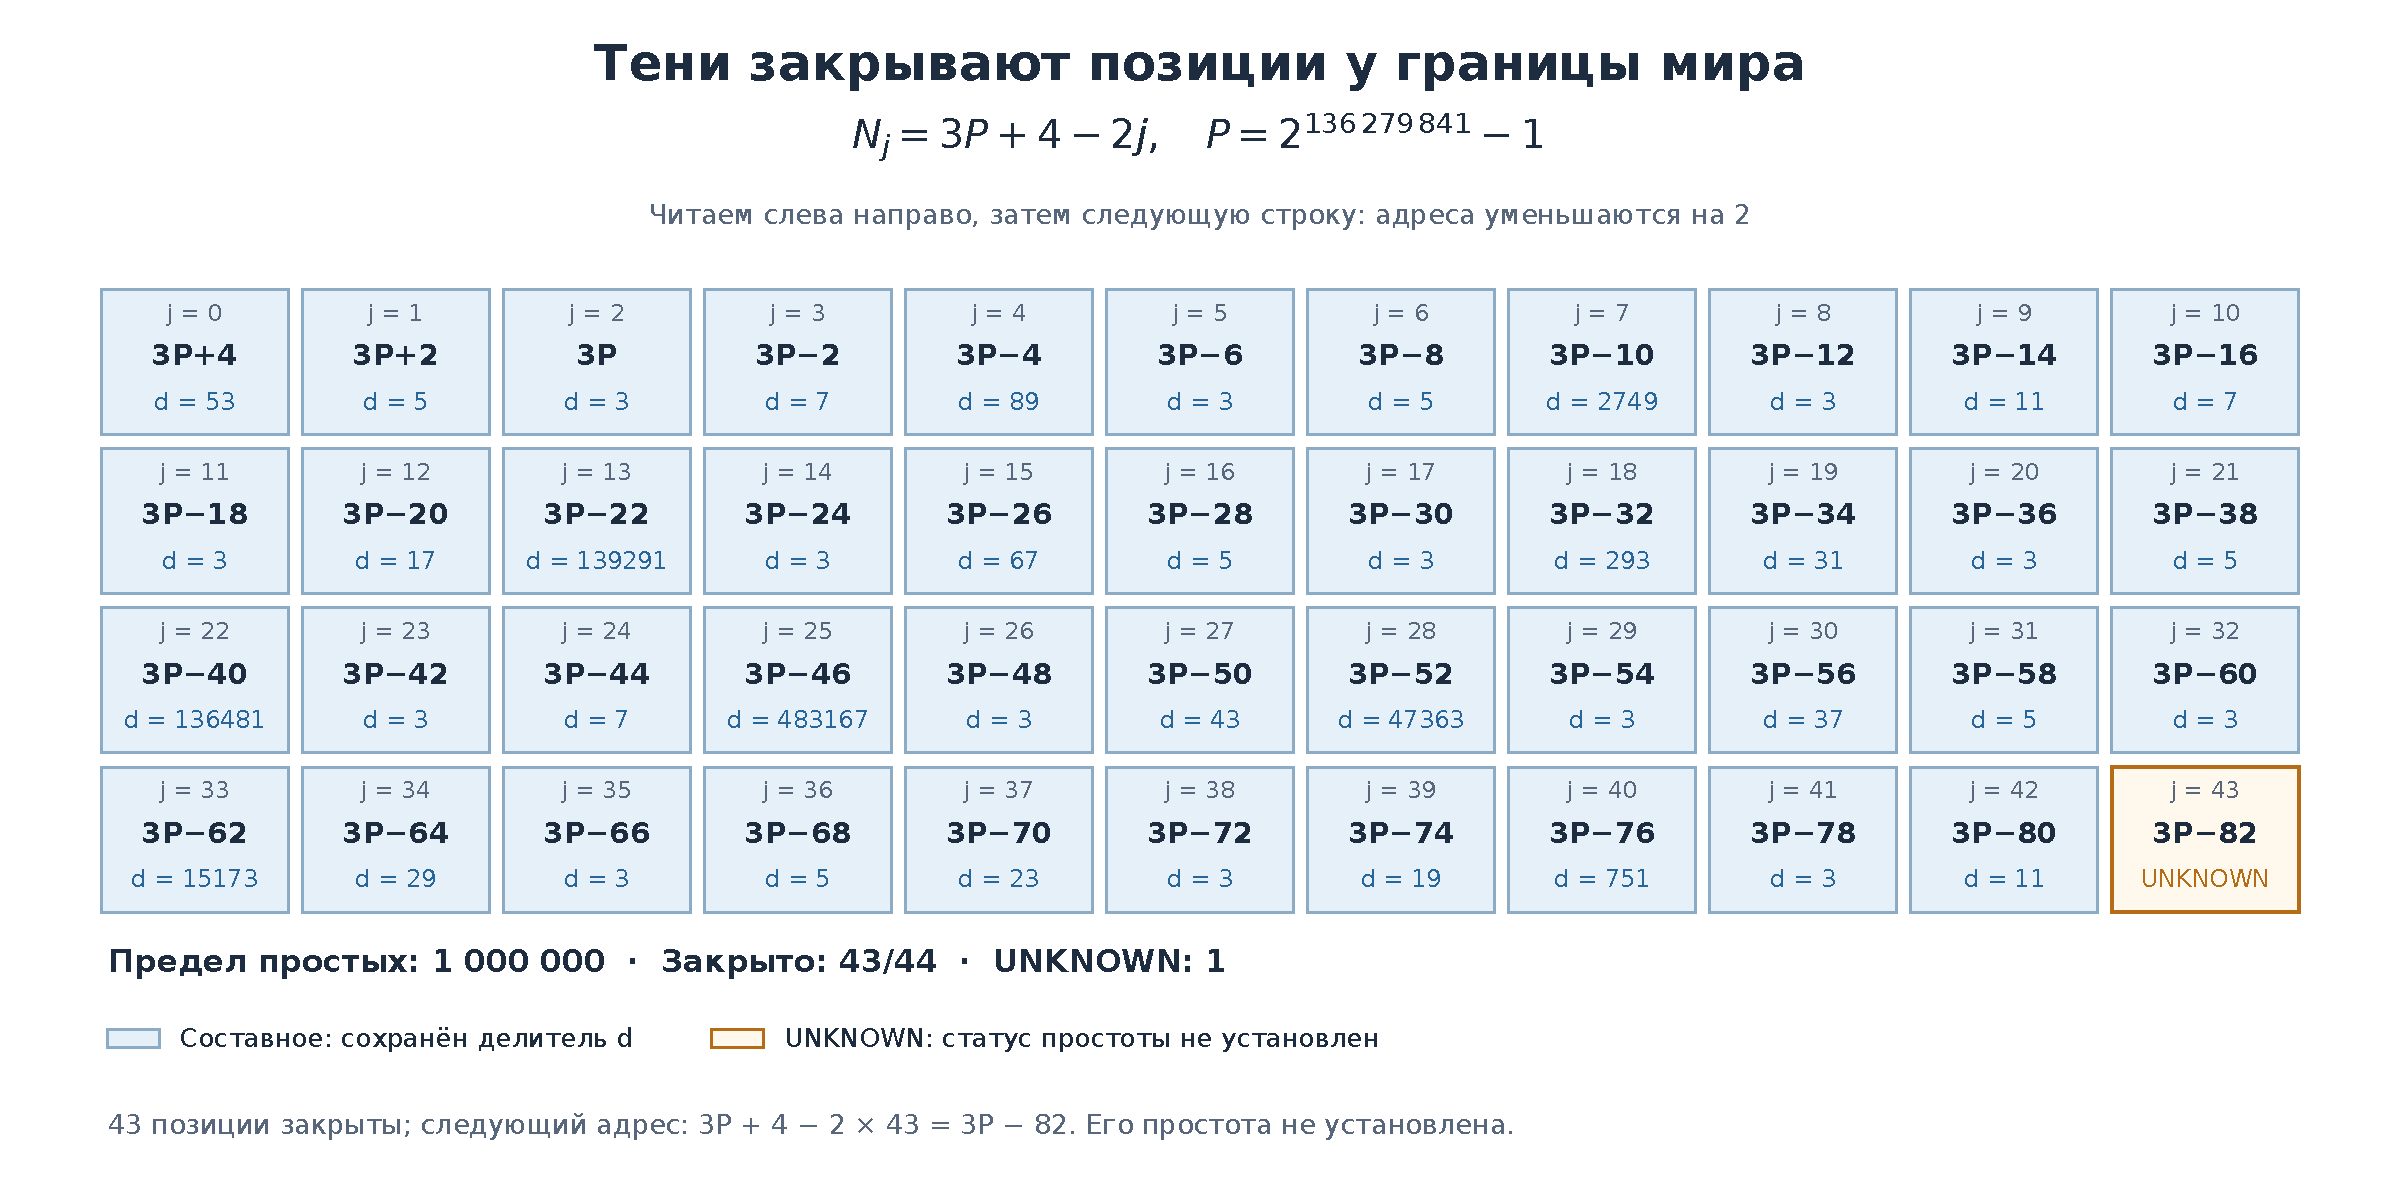
\includegraphics[width=\linewidth]{record_window.pdf}
\end{figure}

\textbf{Статус.} У $3P-82$ не найдено простого делителя до миллиона. Его простота не установлена. Это первый оставшийся кандидат при движении от $R$ вниз; он не объявляется ближайшим простым после $P$. Закрытый участок справа доказан точными делителями и повторно воспроизведён.

\textbf{Поглощение старых теней подтверждено при самом $P$.} Для тех же 1500 адресов вычислены \emph{все} степени простых до $Y=10^6$. Из 78\,497 нечётных простых непустой след имеют 1161. Максимальная длина полного малого делителя $D_Y(N_j)$ -- только 80 бит; максимальная степень простого равна 6. Все адреса $N_j>2^{136\,279\,841}$. Поэтому $D_Y(N_j)<N_j$ подтверждено точно, без построения огромных чисел.

Следовательно, \textbf{тени 5, 7, 13, 1013 и всех остальных простых до миллиона поглощены более поздними осями в этом окне}. Наибольшее малое произведение получено при $j=17$:
\[
 D=D_Y(N_{17})=1152208172826291812625387.
\]
Так как $N_{17}=3P-30>D^2$, любой его простой делитель не превосходит $N_{17}/D$. Для всего окна имеем
\[
 \boxed{10^6<a_*\le\frac{3P-30}{D}<2{,}603697\cdot10^{-24}P.}
\]
Это строгие границы начала полного суффикса исходных осей; промежуток остаётся огромным. Его длина не является объёмом разреженного мира правил. Поздние владельцы по отдельности не найдены. У 119 адресов $D_Y=1$, что сохраняет статус \code{UNKNOWN}: если адрес прост, большой простой делитель равен ему самому и не является покрывающей осью мира $P$. Новый сертификат доказывает поглощение старых слоёв, но не простоту кандидатов.

\section{Ресурсы, предел текущей проверки и запуск}

Ресурсы зафиксированы программой \code{src/resource_audit.py}; исходный снимок находится в \code{data/resources.json}.
\begin{center}
\begin{tabularx}{\linewidth}{@{}lX@{}}
\toprule
Параметр & Доступная среда\\
\midrule
Модель CPU, сообщаемая средой & Intel Xeon Platinum 8573C\\
CPU & 9 видимых логических CPU; общая квота 8 CPU\\
Замеры скорости & Привязка к одному логическому CPU\\
Оперативная память & Лимит 8 ГиБ\\
Swap & Активный swap не обнаружен\\
GPU & Устройства GPU среде не предоставлены\\
Среда исполнения & Linux x86\_64, Python 3.12.14\\
\bottomrule
\end{tabularx}
\end{center}

Двоичная запись $P$ требует 17\,034\,981 байт, около 16,25 МиБ без накладных расходов представления. Сам размер числа помещается в память. Для реализованной полной проверки перебором барьер -- количество возможных делителей.

Для $R=3P+4$ получаем $\log_{10}\sqrt R\approx20\,512\,160{,}21$. По асимптотике $\pi(x)\sim x/\ln x$ число простых до этой границы оценивается как
\[
 \pi(\sqrt R)\approx3{,}44\cdot10^{20\,512\,152}.
\]
Даже условный полный проход со скоростью $10^{12}$ проверок в секунду дал бы около $1{,}09\cdot10^{20\,512\,133}$ лет. Это оптимистическая модель \emph{исчерпывающего прохода}, не измеренная скорость и не нижняя граница для всех алгоритмов простоты. \textbf{Она не вычисляет глубину ряби и не ограничивает все способы сжатия правил.} Кандидат с доступным малым делителем исключается намного раньше.

\textbf{Критика.} Локальное покрытие дёшево, но оно ещё не заменяет сертификат простоты оставшегося кандидата. Увеличение числа ядер или памяти не делает описанный полный проход практическим. Нужен доказанный способ дальнейшего сокращения работы или иной точный сертификат. Получение нового простого рекордного размера этой реализацией не продемонстрировано.

\textbf{Запуск из корня пакета:}
\begin{quote}\small\ttfamily
python src/run\_all.py\\
python src/reproduce.py --benchmark\\
python src/make\_figures.py --video\\
python src/build\_paper.py
\end{quote}
Первая команда проверяет арифметику и воспроизводит локальный опыт; расчёты используют стандартную библиотеку Python. Канонический замер требует Linux/WSL. Для рисунков нужны Matplotlib и Pillow, для видео -- FFmpeg, для PDF -- XeLaTeX и шрифты DejaVu. Команды и точные границы проверок приведены в README.

\begingroup\small
\begin{thebibliography}{4}
\setlength{\itemsep}{3pt}
\setlength{\parskip}{1pt}
\bibitem{hac} A. Menezes, P. van Oorschot, S. Vanstone.
\emph{Handbook of Applied Cryptography}, гл. 4, §§4.23--4.25.
\url{https://cacr.uwaterloo.ca/hac/about/chap4.pdf}.
\bibitem{sorenson} J. Sorenson, J. Webster.
\emph{Strong Pseudoprimes to Twelve Prime Bases}, 2015.
\url{https://arxiv.org/abs/1509.00864}.
\bibitem{primesieve} K. Walisch. \emph{primesieve}: официальный код и описание.
\url{https://github.com/kimwalisch/primesieve}.
\bibitem{gimps} GIMPS. Сообщение о простом $2^{136279841}-1$, 2024.
\url{https://www.mersenne.org/primes/?press=M136279841}.
\end{thebibliography}
\endgroup
\end{document}
